\subsection{Modeling Validation}
During the Machine Learning evaluation phase, variants including LightGBM, XGBoost, and CatBoost were evaluated under a constrained temporal holdout / stress-validation setup, with March 2026 treated as the stress validation period. Table \ref{tab:model_comp} compares these models across the overall segment using WMAPE (Weighted Mean Absolute Percentage Error).

\begin{table}[H]
\centering
\small
\caption{Model Comparison Metrics (Overall)}
\label{tab:model_comp}
\resizebox{\linewidth}{!}{
\begin{tabular}{lllll}
\toprule
\textbf{Model Variant} & \textbf{MAE} & \textbf{RMSE} & \textbf{WMAPE} & \textbf{Bias Ratio} \\
\midrule
LightGBM\_monthly\_minimal\_features & 61.35 & 116.83 & 0.4744 & -0.1653 \\
XGBoost\_monthly\_minimal\_features & 64.54 & 107.33 & 0.4990 & 0.0178 \\
\textbf{CatBoost\_monthly\_minimal\_features} & 55.48 & 97.88 & \textbf{0.4290} & -0.0036 \\
LightGBM\_monthly\_extended\_features & 67.44 & 124.95 & 0.5215 & -0.3801 \\
XGBoost\_monthly\_extended\_features & 62.28 & 105.84 & 0.4816 & -0.2373 \\
CatBoost\_monthly\_extended\_features & 59.27 & 108.35 & 0.4583 & -0.2863 \\
LightGBM\_weekly\_minimal\_features & 31.18 & 49.16 & 0.9460 & 0.3621 \\
XGBoost\_weekly\_minimal\_features & 29.41 & 48.62 & 0.8923 & 0.2648 \\
CatBoost\_weekly\_minimal\_features & 31.08 & 52.62 & 0.9431 & 0.2770 \\
LightGBM\_weekly\_extended\_features & 29.28 & 47.74 & 0.8884 & 0.2409 \\
XGBoost\_weekly\_extended\_features & 29.17 & 48.12 & 0.8850 & 0.2616 \\
CatBoost\_weekly\_extended\_features & 29.33 & 49.38 & 0.8901 & 0.2530 \\
\bottomrule
\end{tabular}
}
\begin{flushleft}
\footnotesize \textit{Note.} WMAPE is the primary normalized metric for comparison.
\end{flushleft}
\end{table}


\begin{table}[H]
\centering
\small
\caption{Best ML Forecast vs Group-Share Base}
\label{tab:cb_vs_base}
\resizebox{\linewidth}{!}{
\begin{tabular}{llll}
\toprule
\textbf{Method} & \textbf{Q2 Forecast Quantity} & \textbf{Q2 Forecast Revenue (VND)} & \textbf{Interpretation} \\
\midrule
Group-Share Base & 37,596 & 60,914,780,907 & Primary operational baseline (Base scenario) \\
CatBoost\_monthly\_minimal\_features & 51,640 & 85,652,196,872 & Best ML validation variant (reference only) \\
\bottomrule
\end{tabular}
}
\begin{flushleft}
\footnotesize \textit{Note.} Group-Share Base is taken from the Base scenario only, not the sum of Conservative, Base, and Aggressive scenarios. CatBoost is shown as a reference ML forecast and is not the official planning baseline.
\end{flushleft}
\end{table}


CatBoost\_monthly\_minimal\_features achieved the lowest validation WMAPE among the evaluated ML variants; however, Group-Share remains the primary operational forecast.

It is important to interpret these metrics with caution. While weekly models utilize a larger volume of data points, their WMAPE is often worse than monthly models because demand is highly volatile at the weekly grain, leading to higher variance in error margins. Furthermore, absolute metrics like MAE and RMSE are not directly comparable between weekly and monthly models due to the differing magnitudes of aggregated volumes.

\subsection{Machine Learning Insights}
Despite the aforementioned volatility, the Machine Learning experiments extracted valuable feature importance signals. Table \ref{tab:feat_imp} highlights the core features driving the ML algorithms.

\begin{table}[H]
\centering
\small
\caption{Top ML Features by Importance}
\label{tab:feat_imp}
\resizebox{\linewidth}{!}{
\begin{tabular}{lll}
\toprule
\textbf{Feature} & \textbf{Avg Importance} & \textbf{Interpretation} \\
\midrule
qty\_roll\_mean\_4w & 92.7124 & Rolling weekly demand momentum \\
qty\_lag\_2w & 72.8203 & Two-week lagged demand signal \\
qty\_lag\_1 & 65.3358 & Immediate short-term demand momentum \\
qty\_lag\_4w & 65.2720 & Four-week lagged demand signal \\
line\_id\_clean & 56.1627 & Product hierarchy / category proxy \\
\bottomrule
\end{tabular}
}
\begin{flushleft}
\footnotesize \textit{Note.} Feature importance averaged across LightGBM/XGBoost variants. Feature importance is directional and should not be interpreted causally.
\end{flushleft}
\end{table}


\subsection{Business Scenario Planning}
Due to ML volatility caused by the March shock, Group-Share remains the primary operational forecast. Table \ref{tab:scenario} and Figure \ref{fig:scenario} summarize the Group-Share allocation scenarios for Q2 2026.

\begin{table}[H]
\centering
\small
\caption{Scenario Delta and Planning Implication}
\label{tab:scenario}
\resizebox{\linewidth}{!}{
\begin{tabular}{llllll}
\toprule
\textbf{Scenario} & \textbf{Q2 Quantity} & \textbf{Q2 Revenue (VND)} & \textbf{Delta Qty vs Base} & \textbf{Delta Revenue vs Base (VND)} & \textbf{Planning Use} \\
\midrule
Conservative & 31,956 & 51,776,591,623 VND & -5,640 & -9,138,189,284 VND & Financial risk control \\
Base & 37,596 & 60,914,780,907 VND & 0 & 0 VND & Primary baseline \\
Aggressive & 42,953 & 69,594,440,480 VND & +5,357 & +8,679,659,573 VND & Capacity buffer \\
\bottomrule
\end{tabular}
}
\begin{flushleft}
\footnotesize \textit{Note.} Conservative controls financial downside risk. Aggressive prepares for sales upside.
\end{flushleft}
\end{table}


\begin{figure}[H]
\centering
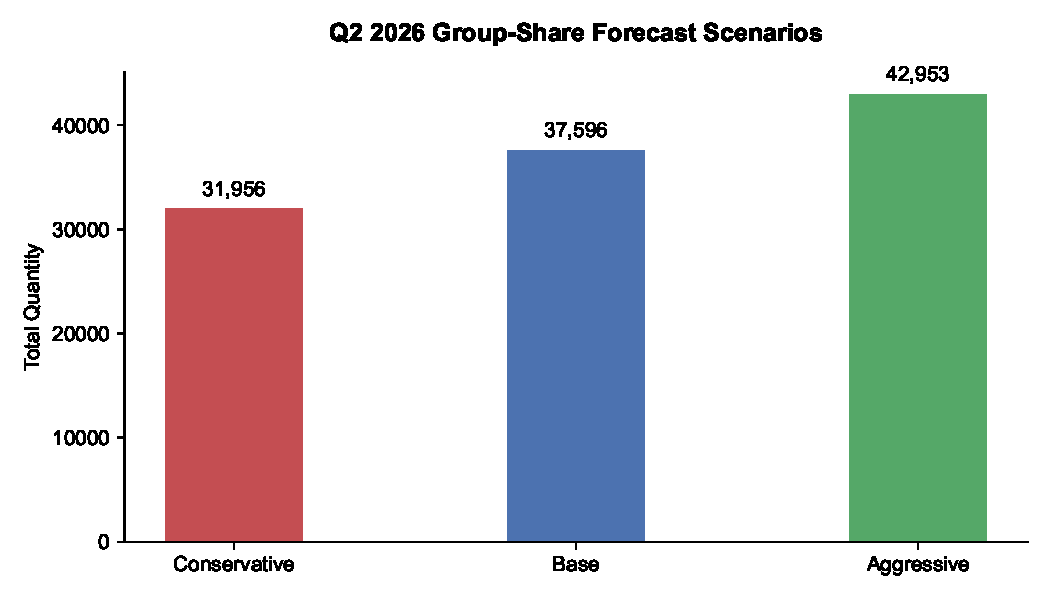
\includegraphics[width=0.85\textwidth]{../figures/en/scenario_forecast.pdf}
\caption{Q2 2026 Group-Share Forecasted Quantity Scenarios}
\label{fig:scenario}
\end{figure}

The Base scenario anchors standard material procurement planning. The Aggressive scenario serves as a strategic capacity buffer for supply chain resilience. Finally, the Conservative scenario assists executive management in controlling cash flow and inventory risks.
\FloatBarrier
